\documentclass[12pt]{article}
\pdfoutput=1
\usepackage[T2A]{fontenc}
\usepackage[utf8]{inputenc}
\usepackage[english, russian]{babel}
%\usepackage{NotesTex_rus}
\usepackage{a4wide}
\usepackage{amsmath,amsfonts,amssymb,amsthm,mathtools} 
\usepackage{wasysym}
\usepackage{indentfirst}
\usepackage{a4wide}
\usepackage{mathtools}
\usepackage{dsfont}
\usepackage{float} 
\usepackage{hyperref}


\DeclarePairedDelimiter{\norm}{\lVert}{\rVert} 

\newtheorem{theorem}{Теорема}
\newtheorem{note}{Замечание}
\newtheorem{statement}{Утверждение}
\newtheorem{definition}{Определение}

\DeclareMathOperator{\sgn}{sgn}

%Заголовок
%\usepackage{graphix}

\begin{document}
\thispagestyle{empty}
\begin{center}
\vspace{-3cm}

\includegraphics[width=0.5\textwidth]{msu.eps}\\

{\scshape Московский государственный университет имени М.~В.~Ломоносова}\\
Факультет вычислительной математики и кибернетики \\
Кафедра системного анализа

\vfill
{\LARGE Курсовая работа}
\vspace{3cm}

{\Huge\bfseries <<Исследование нелинейных динамических систем на плоскости>>}
\end{center}
\vspace{1cm}
\begin{flushright}
\large
\textit{Студент 315 группы}\\
Г.~А.~Юшков \\
\vspace{5mm}
\textit{Преподаватель}\\
к.ф.-м.н., доцент И.~В.~Востриков
\end{flushright}
\vfill
\begin{center}
Москва, 2022
\end{center}
\makeatother

\newpage
\tableofcontents

\newpage
\section{Постановка задачи}
Дана система уравнений:
\begin{equation} \label{sys1}
    \begin{cases}
        \frac{du}{dt} = 1 - (b+1)u + au^2v,\\
        \frac{dv}{dt} = bu - au^2v,
    \end{cases}
    (u,v) \in \mathbb{R}^2_+, ~ a, b > 0.
\end{equation}
Необходимо:
\begin{enumerate}
    \item Дать биологическую интерпретацию характеристик системы.
    \item Ввести новые безразмерные переменные, максимально уменьшив число входящих параметров. Выбрать два свободных параметра. Если число параметров больше двух, то считать остальные параметры фиксированными.
    \item Найти неподвижные точки системы и исследовать их характер в зависимости от значений параметров. Результаты исследования представить в виде параметрического портрета системы.
    \item Для каждой характерной области параметрического портрета построить фазовый портрет. Дать характеристику поведения системы в каждом из этих случаев.
    \item Исследовать возможность возникновения предельного цикла. В положительном случае найти соответствующее первое ляпуновское число. Исследовать характер предельного цикла (устойчивый, неустойчивый, полуустойчивый).
    \item Дать биологическую интерпретацию полученным результатам.
\end{enumerate}

\newpage
\section{Биологическая интерпретация системы}
Система моделирует скорость изменения  концентраций веществ в системе химических реакций:
\begin{equation} \label{syschem}
    \begin{cases}
        A \to X, \\
        2X + Y \to 3X, \\
        B + X \to Y + D, \\
        X \to E,
    \end{cases}
\end{equation} 
В данной системе A и B - исходные вещества, концентрация которых достаточно велика, чтобы считаться постоянной; X И Y - промежуточные вещества, получающиеся в ходе преобразования исходных; D и E - конечные продукты реакции. Подразумевается, что вещества D и E не вступают в реакции в данных условиях. Также подразумевается, что каждая из реакций в системе (\ref{syschem}) имеет свои условия протекания (например, освещение, нагревание, и т.д), которые отдельно не указываются в силу ненадобности для изучения математической стороны задачи.
\section{Введение безразмерных параметров}
Требования второго пункта задания для нащей задачи уже выполнены, однако покажем, как происходит переход от текстового описания системы (\ref{syschem}) к системе дифференциальных уравнений (\ref{sys1}). Запишем изначальную версию уравнения, вытекающую из закона действующих масс, который гласит, что скорость реакции пропорциональна произведению концентраций реагентов:
\begin{equation}
    \begin{cases}
        \frac{dX}{dt} = k_1A - k_2BX + k_3X^2Y - k_4X,\\
        \frac{dY}{dt} = k_2BX - K_3X^2Y.
    \end{cases}
\end{equation}
Здесь X, Y, A, B - концентрации соответствующих веществ из системы (\ref{syschem}). Проведём замену переменных:
\begin{equation}
    \begin{cases}
        x = \sqrt{\frac{k_3}{k_4}}X,\\
        y = \sqrt{\frac{k_3}{k_4}}Y,\\
        \tau = k_4t,\\
        a = \sqrt{\frac{k_1^2k_3}{k_4^3}}A,\\
        b = \frac{k_2}{k_4}B.
    \end{cases}
\end{equation}
Тогда система примет вид:
\begin{equation} \label{syschemcommon}
    \begin{cases}
        \frac{dx}{d\tau} = a - (b + 1)x + x^2y,\\
        \frac{dy}{d\tau} = bx - x^2y.
    \end{cases}
\end{equation}
Несложно заметить, что дальнейшее приведение проводится масштабированием параметров a и b.

\newpage
\section{Исследование неподвижных точек}
\subsection{Поиск неподвижных точек}
\begin{definition}
    Точка $x_0 \in \mathbb{R}^n$ называется неподвижной точкой динамической системы $\dot{x_i} = f_i(x_1, ..., x_n), i = \overline{1,n}, f = (f_1, ..., f_n)$, если $f(x_0) = 0$.
\end{definition}
Для нахождения неподвижных точек решим систему:
\begin{equation}
    \begin{cases}
        0 = 1 - (b+1)u + au^2v,\\
        0 = bu - au^2v.
    \end{cases}
\end{equation}
Второе уравнение равносильно тому, что либо $u=0$, что, очевидно, не подходит для первого уравнения, либо $v = \frac{b}{au}$. В таком случае подстановкой $v$ в первое уравнение получаем: $u = 1$, $v = \frac{b}{a}$. Значит, система имеет ровно 1 неподвижную точку: $\left(1, \frac{b}{a}\right)$.
\subsection{Тип и устойчивость неподвижных точек}
\begin{theorem} \label{th1}
    Пусть $u^*$ - положение равновесия, а $J(u)$ - матрица Якоби исследуемой динамической системы. Тогда неподвижная точка $u^*$ асимптотически устойчива, если все собственные значения $\lambda_1, \lambda_2, ..., \lambda_n$ матрицы Якоби, вычисленные в точке $u^*$, таковы, что $Re(\lambda_i) < 0$, $i = 1, ..., n$. Если хотя бы одно собственное значение $\lambda_i$ таково, что $Re(\lambda_i) > 0$, то неподвижная точка $u^*$ неустойчива.
\end{theorem}
Рассмотрим матрицу Якоби системы (\ref{sys1}).
$$
    J(u,v) = 
    \begin{bmatrix}
        -(b+1) + 2auv & b - 2auv \\
        au^2 & -au^2
    \end{bmatrix}.
$$
Получаем:
$$
    J\left(1,\frac{b}{a}\right) = 
    \begin{bmatrix}
        b-1 & -b \\
        a & -a
    \end{bmatrix}.
$$
Найдём собственные значения:
$$
    det\left(J\left(1, \frac{b}{a}\right) - \lambda I\right) = 0.
$$
\begin{center}
    $\Updownarrow$
\end{center}
$$
    (b - 1 - \lambda)(-a-\lambda) + ab = 0.
$$
\begin{center}
    $\Updownarrow$
\end{center}
\begin{equation}\label{characteristic}
    \lambda^2 - (b - a - 1)\lambda + (b-1)(-a) + ab = \lambda^2 - (b - a - 1)\lambda + a = 0.
\end{equation}
\begin{center}
    $\Updownarrow$
\end{center}
\begin{equation}
    \lambda_{1,2} = \frac{b - a - 1 \pm \sqrt{(b - a - 1)^2 - 4a}}{2}.
\end{equation}
Простым разбором случаев по знаку выражения $b - a - 1$ устанавливается, что:
\begin{equation}
    \begin{cases}
        b - a - 1 > 0 - \text{неподвижная точка неустойчива},\\
        b - a - 1 < 0 - \text{неподвижная точка асимптотически устойчива},\\
        b - a - 1 = 0 - \text{теорема неприменима}.
    \end{cases}
\end{equation}
Заметим, что:
$$
    \lambda_1\lambda_2 = \frac{(b - a - 1)^2 - ((b - a - 1)^2 - 4a)}{4} = \frac{4a}{4} = a > 0 ~\forall a,b>0.
$$
Тип неподвижной точки зависит только от знака выражения под корнем, это следует из положительности произведения собственных значений. Таким образом, получаем:
\begin{equation}
    \begin{cases}
        (b - a - 1)^2 - 4a \geqslant 0 - \text{узел},\\
        (b - a - 1) = 0 - \text{центр},\\
        (b - a - 1)^2 - 4a < 0, (b - a - 1) \neq 0 - \text{фокус}.
    \end{cases}
\end{equation}
Параметрический портрет системы представлен на графике ниже (НУ - неустойчивый узел, НФ - неустойчивый фокус, УФ - устойчивый фокус, УУ - устойчивый узел, центру соответствует синяя прямая на графике):
\begin{figure} [H]
    \begin{center}
    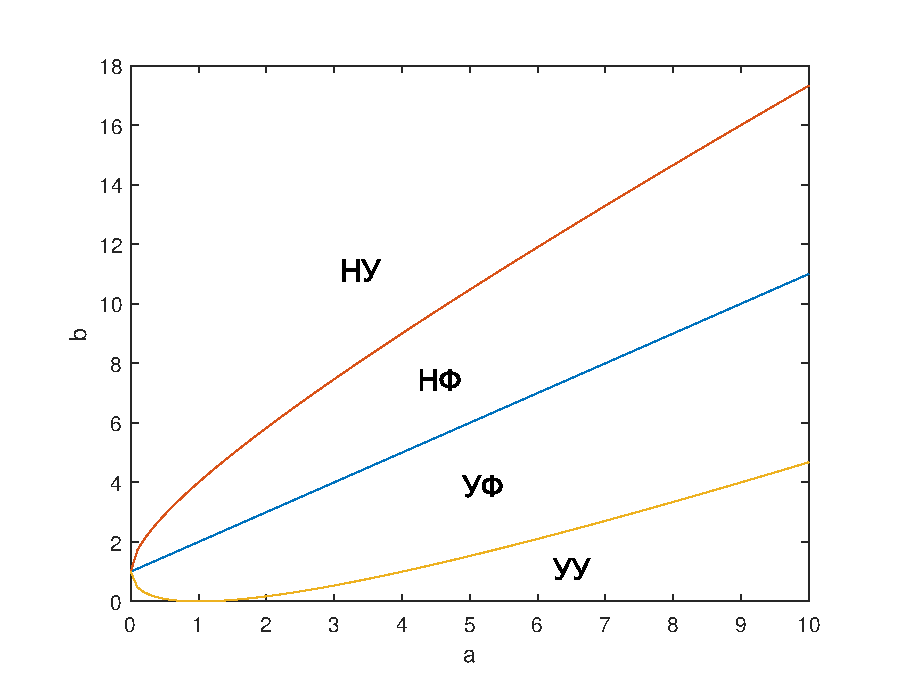
\includegraphics[width=0.8\textwidth]{paramport.eps}
    \caption{Параметрический портрет системы.}
    \label{pic1}
    \end{center}
\end{figure}

\newpage
\section{Фазовые портреты}
Построим фазовые портреты для каждой из областей.
\subsection{Неустойчивый узел}
    Для случая неустойчивого узла возьмём $a = 1, b = 5$. Точка $\left(1, 5\right)$ - неустойчивый узел.
    \begin{figure} [H]
        \begin{center}
        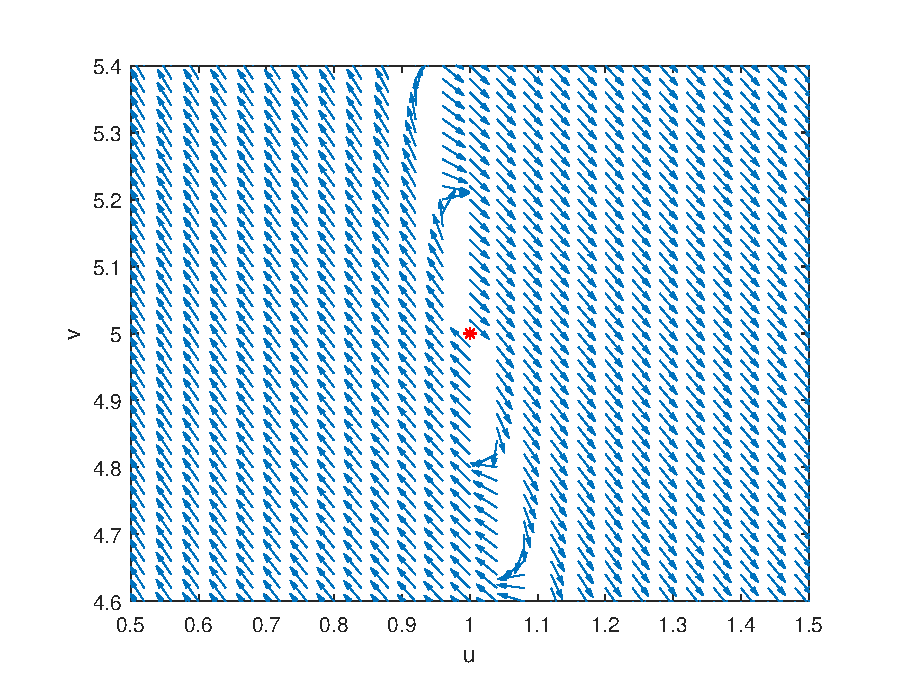
\includegraphics[width=1\textwidth]{phaseport1.eps}
        \caption{Фазовый портрет системы. Неустойчивый узел.}
        \label{pic2}
        \end{center}
    \end{figure}
\newpage
\subsection{Неустойчивый фокус}
    Для случая неустойчивого фокуса возьмём $a = 1, b = 3$. Точка $\left(1, 3\right)$ - неустойчивый фокус.
    \begin{figure} [H]
        \begin{center}
        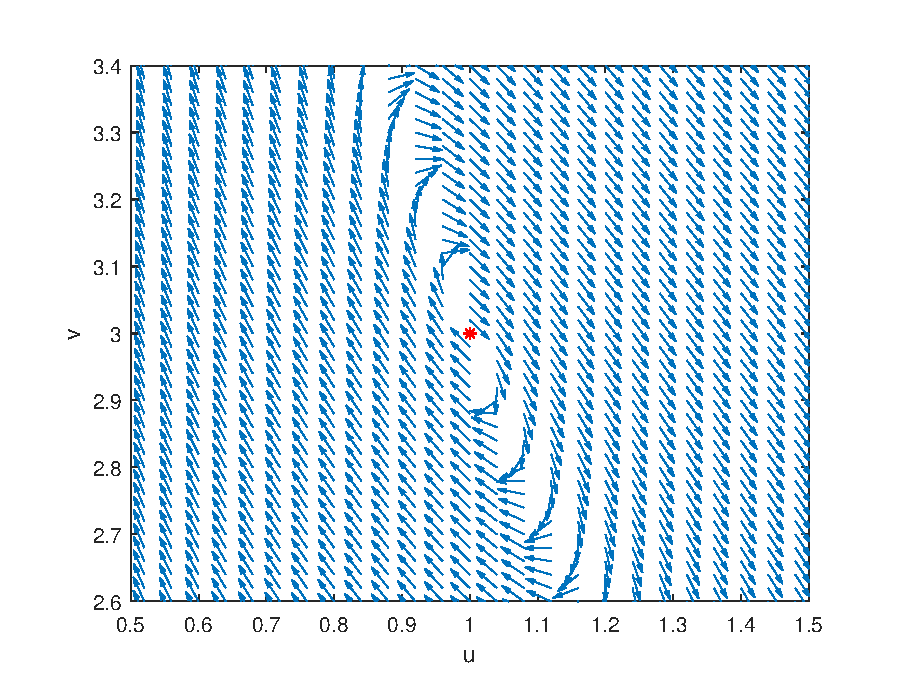
\includegraphics[width=1\textwidth]{phaseport2.eps}
        \caption{Фазовый портрет системы. Неустойчивый фокус.}
        \label{pic3}
        \end{center}
    \end{figure}
\newpage
\subsection{Устойчивый фокус}
    Для случая устойчивого фокуса возьмём $a = 1, b = 1$. Точка $\left(1, 1\right)$ - устойчивый фокус.
    \begin{figure} [H]
        \begin{center}
        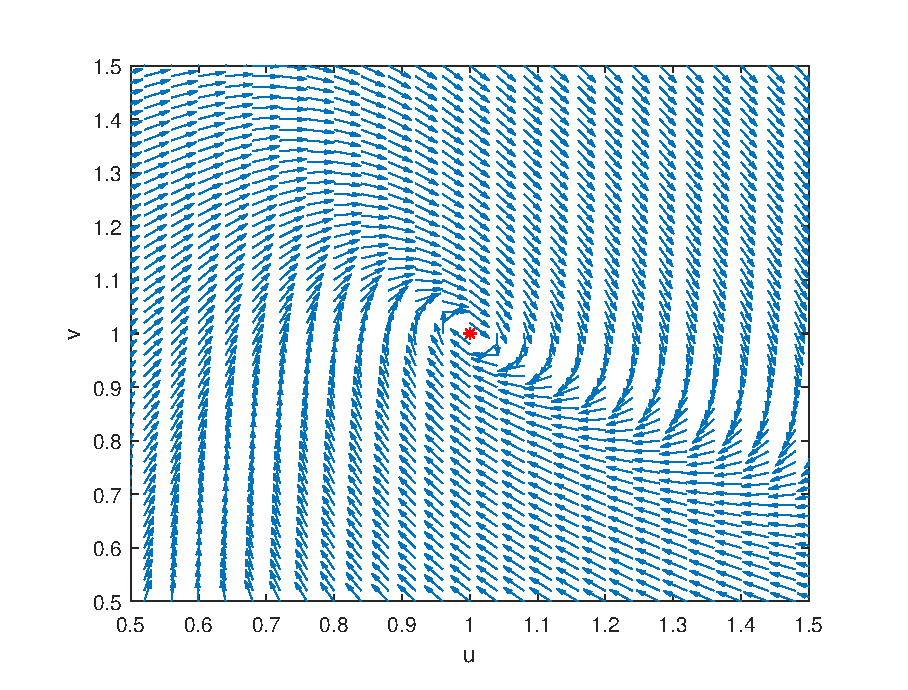
\includegraphics[width=1\textwidth]{phaseport3.eps}
        \caption{Фазовый портрет системы. Устойчивый фокус.}
        \label{pic4}
        \end{center}
    \end{figure}
\newpage
\subsection{Устойчивый узел}
    Для случая устойчивого узла возьмём $a = 7, b = 1$. Точка $\left(1, \frac{1}{7}\right)$ - устойчивый узел.
    \begin{figure} [H]
        \begin{center}
        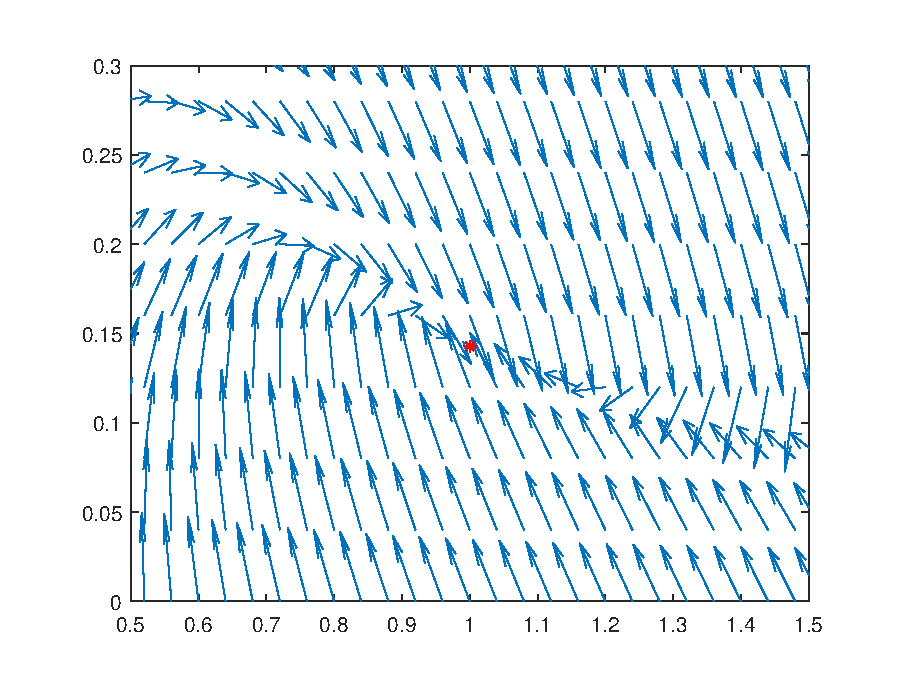
\includegraphics[width=1\textwidth]{phaseport4.eps}
        \caption{Фазовый портрет системы. Устойчивый узел.}
        \label{pic5}
        \end{center}
    \end{figure}

\newpage
\section{Возникновение предельного цикла}
\begin{definition}
    Бифуркация положения равновесия, соответствующая появлению собственных чисел $\lambda_{1,2} = \pm i\omega_0$, где $\omega_0 > 0$, называется бифуркацией Пуанкаре-Андронова-Хопфа или бифуркацией рождения цикла.
\end{definition}
Таким образом, необходимым условием наличия предельного цикла является следующее равенство для собственных значений матрицы $J\left(1, \frac{b}{a}\right)$:
$$
    \lambda_{1,2} = \pm iw, w > 0
$$
Положим для краткости: $c = b - a - 1$. Тогда характеристический многочлен примет вид (см. выражение (\ref{characteristic})):
$$
    \lambda^2 - c\lambda + a = 0, ~ a >0 ~ c \in\mathbb{R}.
$$
Подставим $\lambda = iw$. Получим:
$$
    (iw)^2 - c(iw) + a = 0.
$$
\begin{center}
    $\Updownarrow$
\end{center}
$$
    (a - w^2) - i(cw) = 0.
$$
\begin{center}
    $\Updownarrow$
\end{center}
\begin{equation}
    \begin{cases}
        w^2 = a,\\
        c = 0.
    \end{cases}
\end{equation}
\begin{center}
    $\Updownarrow$
\end{center}
\begin{equation}
    \begin{cases}
        w = \pm \sqrt{a},\\
        b = a + 1.
    \end{cases}
\end{equation}
Видно, что данный результат мы уже получали ранее, когда выясняли типы неподвижных точек, хотя тогда мы явно не вычисляли собственные значения. Произведём в изначальной системе замену $b = a + 1$. Получим систему, зависящую только от параметра $a > 0$. В таком случае воспользуемся теоремой:
\begin{theorem}
    Любая двумерная однопараметрическая система $\dot{u} = f(u;\alpha)$, имеющая при достаточно малых $|\alpha|$ положение равновесия $u = 0$ с собственными числами $\lambda_{1,2}(\alpha) = \mu(\alpha) \pm i\omega(\alpha), \mu(0) = 0, \omega(0) = \omega_0 > 0$ и удовлетворяющая условиям невырожденности
    \begin{equation}
        \left.\frac{d}{d\alpha}\mu(\alpha)\right\vert_{\alpha = 0} \neq 0,
    \end{equation}
    \begin{equation}
        l_1(0) = \frac{1}{2\omega_0}Re(ig_{20}(0)g_{11}(0)+\omega_0g_{21}(0)) \neq 0,
    \end{equation}
    где
    $$
        g_{kl}(\alpha) = \left.\frac{\delta^{k+l}}{\delta z^k \delta \bar{z}^{l}} \langle p(\alpha), F(zq(\alpha) + \bar{z}\bar{q}(\alpha)) \rangle\right\vert_{z=\bar{z}=0}
    $$
    в окрестности начала координат локально топологически эквивалентна одной из двух динамических систем
    $$
        \dot{v_1} = \alpha v_1 - v_2 + \sgn{l_1(0) v_1(v_{1}^{2}+v_{2}^{2}}),
    $$
    $$
        \dot{v_2} = v_1 + \alpha v_2 + \sgn{l_1(0) v_2(v_{1}^{2}+v_{2}^{2}}).
    $$
\end{theorem}
В нашем случае при $b = a + 1$ неподвижной будет точка $P = \left(1, \frac{a+1}{a}\right)$. Проведём замену переменных, соответствуюшую смещению неподвижной точки в начало координат:
\begin{equation}
    \begin{cases}
        u_1 = u - 1,\\
        v_1 = v - 1.
    \end{cases}
\end{equation}
Запишем получившуюся систему:
\begin{equation}
    \begin{cases}
        \frac{du_1}{dt} = 1 - (a+2)(u_1 + 1) + a(u_1 + 1)^2\left(v_1 + \frac{a+1}{a}\right),\\
        \frac{dv_1}{dt} = (a+1)(u_1 + 1) + a(u_1 + 1)^2\left(v_1 + \frac{a+1}{a}\right).
    \end{cases}
\end{equation}
Для краткости далее будем сохранять исходные обозначния $u, v$ для новых переменных $u_1, v_1$. Матрица Якоби в неподвижной точке примет вид:
\begin{equation}
    J(0, 0) =
    \begin{bmatrix}
        a & -a - 1 \\
        a & -a
    \end{bmatrix}.
\end{equation}
Как было показано ранее, собственные значения матрицы равны $\lambda_{1,2} = \pm i\sqrt{a}$.
Собственные векторы, соответствующие данным собственным значениям, равны:
$$
    h_1 = \left(1, \frac{a - i\sqrt{a}}{a+1}\right),\\
    h_2 = \left(1, \frac{a + i\sqrt{a}}{a+1}\right).
$$
Вычислим коэффициенты $g_{20}, g_{11}, g_{21}$ и первое ляпуновское число $l_1$ с помощью Matlab. Получим следующий результат:
$$
    l_1(0) = -a(1.357a + 1.401) 
$$
$l_1(0) < 0$, $\forall a > 0$, следовательно, бифуркация суперкритическая (мягкая), с рождением единственного устойчивого предельного цикла (Рис. \ref{limpic}).
\begin{figure}[H]
    \begin{center}
    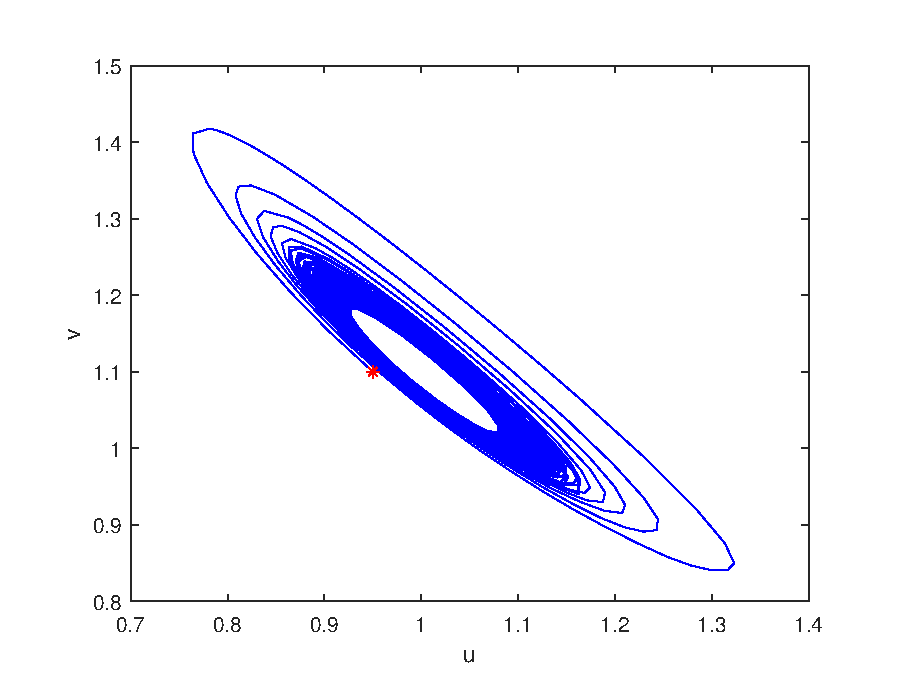
\includegraphics[width=1\textwidth]{limitcycle.eps}
    \caption{Предельный цикл при $a = 10$ Начальная точка обозначена звёздочкой.}
    \label{limpic}
    \end{center}
\end{figure}
\section{Биологическая интерпретация результатов}
Проанализируем полученные результаты:
\begin{itemize}
    \item Для областей НУ/НФ не существует устойчивых точек. Концентрация промежуточных веществ не может стабилизироваться возле какого-то определённого значения на фазовой плоскости $(u, v)$.
    \item Для областей УУ/УФ существует устойчивая точка. Концентрации промежуточных веществ будут стабилизироваться вблизи этой точки.
\end{itemize}

\newpage
\begin{thebibliography}{9}
    \bibitem[1]{} А.\,C.~Братусь, А.\,С.~Новожилов, А.\,П.~Платонов. Динамические системы и модели биологии. — М.: ФИЗМАТЛИТ, 2010.
\end{thebibliography}
\end{document}